\section{Real Domain Tests}
\label{sec:realDomainTests}
	In order to have a better idea of the quality of the methods previously shown I tested them with real instance. These instances are taken from the gerber files avaible from the following online archive:
	\begin{itemize}
		\item \href{https://www.maximintegrated.com/en/design/tools/cad-layout/gerber/}{https://www.maximintegrated.com/en/design/tools/cad-layout/gerber/};
		\item \href{https://www.microchip.com/doclisting/TechDoc.aspx?type=Gerber}{https://www.microchip.com/doclisting/TechDoc.aspx?type=Gerber};
	\end{itemize}

	I explored a dozens of project and select some drill gerber files, from these I made\footnote{This could be done thank to the parser developed by my colleagues Sebastiano Valle and Mirko Bez.} the following \verb|.dat|:
	
	\begin{itemize}
		\item \verb|SC_545|
		\item \verb|MAX_682|
		\item \verb|DS_1120|
	\end{itemize}
	Figure~\ref{fig:SC_545} shows a representation of one of them. The other could be seen from the pdf inside the \verb|RealInstances| folder attached to this report.

	\begin{figure} [h]
		\centering
		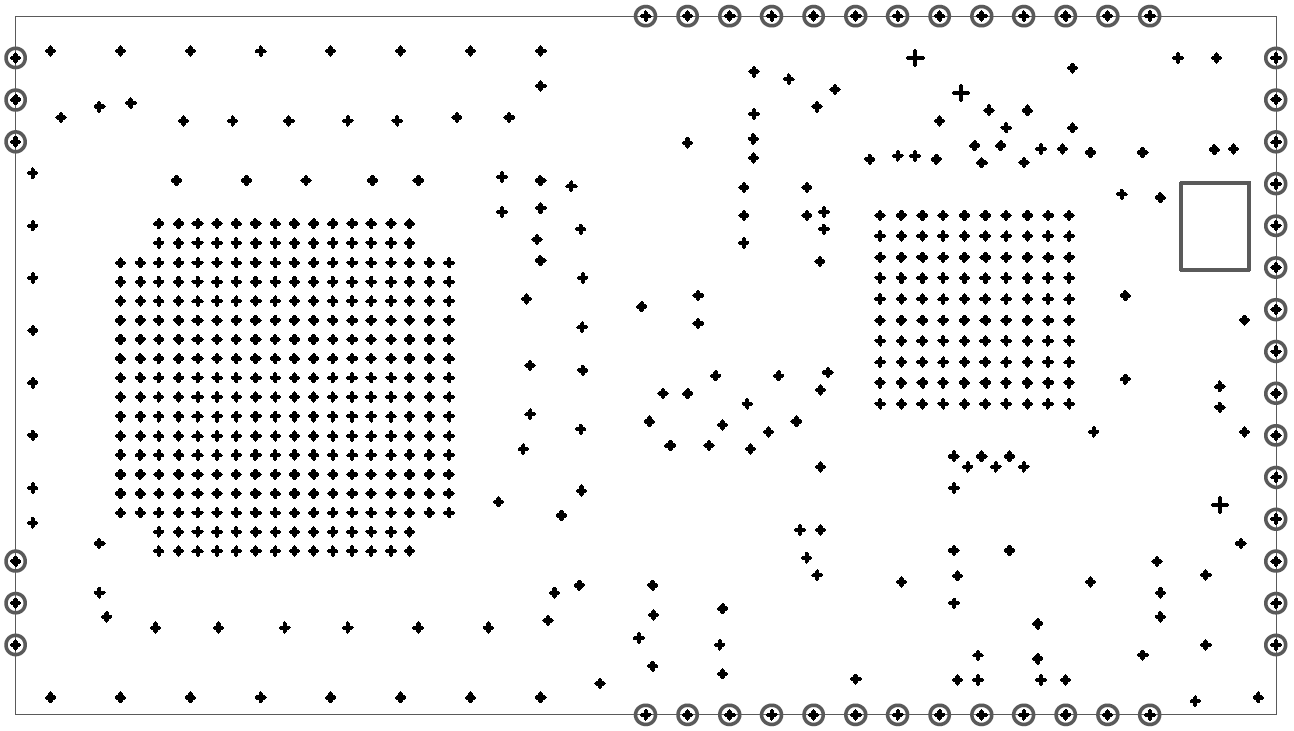
\includegraphics[width=\textwidth]{img/SC_545}
		\caption{The representation of the SC\_545 real instance.}
		\label{fig:SC_545}
	\end{figure}
	
	
	
	\subsection{Results exact method}
		The instances are too huge and the power of computation is too low in order to test the exact method implemented with CPLEX in an amount of time for this project purpose. Neither with a time-out the CPLEX API can give me a intermediate solution in a reasonable amount of time.
		
	%\newpage
	
	\subsection{Results Local Search}
		I run the local search with the \textbf{strategy} explained in the previous section \ref{subsec:results-ls}. As observed in the tests before the First Improvement tend to converge less respect to Best Improvement but this in the case of \verb|SC_545| and \verb|DS_1120| brings better solution but not for \verb|MAX_682| where it takes more time and get a worse solution, same for the average value. Again there are not empirical proves in order to say if First Improvement is better than Best Improvement or vice versa.
		
		\begin{table}[h]
			\centering
			\begin{tabular}{llrrr}
				\toprule
				\textbf{Instance} & \textbf{Feature} & \textbf{Avg Value} & \textbf{Best Value} & \textbf{Tot Time (s)} \\
				\toprule
				\verb|SC_545|  & Best Improv. & 16809.8   & 16440            & 3.59397    \\
				& First Improv. & 16504.8   & 16231            & 5.61317    \\
				\midrule
				\verb|MAX_682| & Best Improv.  & 5350680   & 5187620          & 6.91607    \\
				& First Improv. & 5356200   & 5272060          & 11.5556    \\
				\midrule
				\verb|DS_1120| & Best Improv.  & 17051200   & 16969100      & 39.9405    \\
				& First Improv. & 16921800    & 16742900         & 71.0088   \\
				\bottomrule
			\end{tabular}
		\caption{Local Search result on real instances.}
		\label{fig:ri-results-ls}
		\end{table}
	
	
	\newpage
	
	\subsection{Results Tabu Search}
	
		\subsubsection{Calibration}
			With these new instance the previous calibration is no longer valid. I start from that configuration and I increase the Tabu length.
			
			I made the calibration on \verb|SC_545| instance.
			First I take 8 random initial solution. Then I initialize 4 type of Tabu Search:
			\begin{itemize}
				\item Best Improvement;
				\item Best Improvement with Aspiration Criteria;
				\item First Improvement;
				\item First Improvement with Aspiration Criteria.
			\end{itemize}
			For each type of tabu search I set five different tabu length: 100, 180, 240, 300 and 480. Finally I run each Tabu Search with a maximum time of 30 seconds.  Overall I have $4 \cdot 5 \cdot 8 = 160 $ executions. 
			
			The results are shown in the figure \ref{fig:ri-calibration-sc}.
			
			\begin{figure} [p]
				\centering
				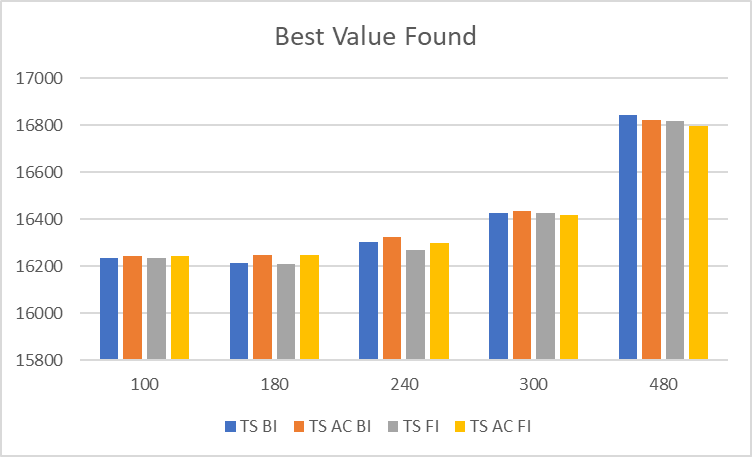
\includegraphics[width=\linewidth]{img/RI-calibration-SC}
				%\caption{Calibration Real Instances - best value found.}
				%\label{fig:ri-calibration-sc}
				\vspace{1cm}
				
				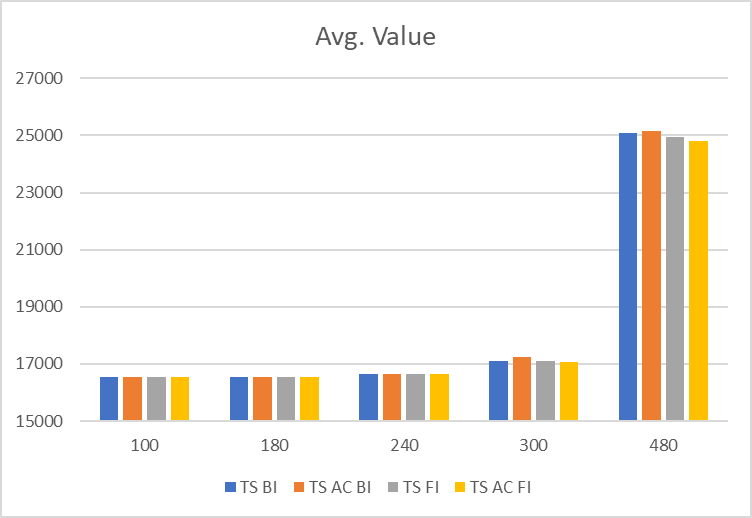
\includegraphics[width=\linewidth]{img/RI-calibration-SC-avg}
				
				\caption{Calibration Real Instances.}
				\label{fig:ri-calibration-sc}
			\end{figure}
		
			From the charts we can observe that there is some particular differences between the types of Tabu Search. 
			Furthermore we can observe that increasing the tabu length decrease the best value found and also the average of value found. This is suspected, in fact, with tabu length equal to 480, we obtain these because with a tabu list too long the program have a performance bottleneck where it checks if a move is a tabu. Hence I start another calibration, only for TS BI AC (choose arbitrarily) with a tabu length equal to 480 and with a maximum time of 300 seconds (5 minutes).
			
			The figure \ref{fig:ri-calibration-optimize} (below) shows with evidence that with more time a larger tabu length is better. If we run a tabu search with tabu length equal to 180 and with a maximum time of 300 seconds we obtain a little improvement but not as the improvement for 480 tabu length case.
			
			
			\paragraph*{Optimize the code} In order to improve the check if a move is a tabu I substitute the tabu list with two data structures. First I use a \verb|std::list| in order to keep the order of moves inserted into the tabu list. With this data structure I can remove the first element and push back at constant time.
			Second I use a \verb|std::set| for check if a move is a tabu in constant time. I use the concatenation of integer \verb|from| and \verb|to| as key. \\
			
			\textbf{N.B.} This optimization could brings better result in all the previously test. For limit of time I use the optimization only from now on. \\
			
			With the implementation I execute again some test with TS BI AC with tabu length 180 and 480. The result is that now with 30 seconds I can achieve a better result with tabu length of 480, also the tabu length of 180 have a better solution. In figure ~\ref{fig:ri-calibration-optimize} are shown the comparison between before and after optimization. 
					
	
			\begin{figure}[p]
				\centering
				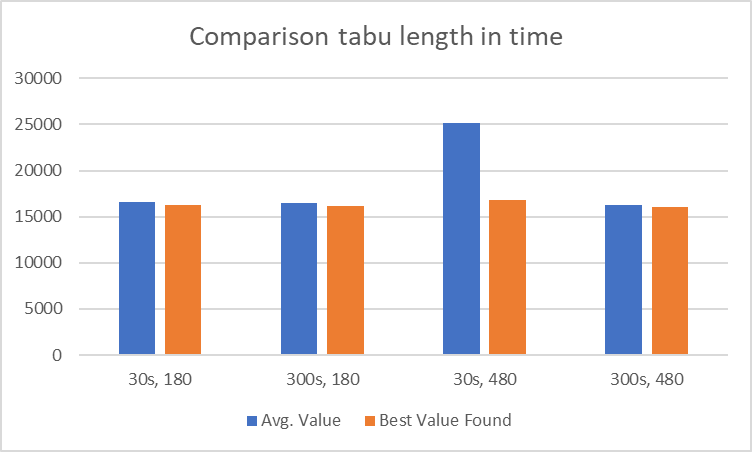
\includegraphics[width=\linewidth]{img/RI-calibration-TabuLengthInTime}
				
				\vspace{1cm}
				
				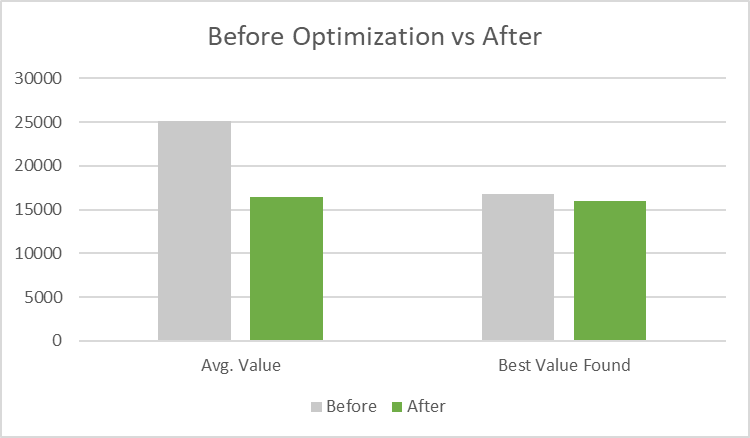
\includegraphics[width=\linewidth]{img/RI-calibration-optimize}
				\caption{Comparison results of TS BI AC with different length and time (above). Result of TS BI AC in 30 seconds, length of 480, without and with optimization of tabu list (below).}
				\label{fig:ri-calibration-optimize}
			\end{figure}
		
\newpage
		

		
	\subsubsection{Calibration (with optimization)}
		I recompute the calibration configured as before. I change a little the tabu lengths tested: 180, 300, 480, 600 and 800. From the results in charts~\ref{fig:ri-calibration-sc-opt} we can see that tabu length of 600 obtains the best value, also in average. The Tabu Search Best Improvement with Aspiration Criteria is the best choice.
		
	\subsubsection{Tests}
		
		For the final tests on real instances I choose to use a Tabu Search with the following configuration:
		\begin{itemize}
			\item Best Improvement;
			\item Aspiration Criteria;
			\item Tabu length of 600;
			\item Maximum time 60 seconds (1 minutes) since the solutions space is much bigger.
			\item Maximum iteration 30,000 ($+\infty$): I use the maximum time as stopping criteria;
		\end{itemize}
		As the previous tests on Tabu Search I use the \textbf{Strategy 2}: I start the tabu search from 8 different random solution and I select the best value found. The total time of computation are 8 minutes. The table~\ref{fig:ri-results-ts} summarize the results.
		
		\begin{table}[hb]
			\centering
			\begin{tabular}{lrrrr}
				\toprule
				\textbf{Solver} & \textbf{Avg Value} & \textbf{Best Value} & \textbf{Avg Time (s)} & \textbf{Tot. Time (s)} \\
				\toprule
				\verb|SC_545|         & 16250.2            & 15991               & 60.0072               & 480.058                \\
				\verb|MAX_682|        & 5276730            & 5115970             & 60.0150               & 480.120                \\
				\verb|DS_1120|        & 35080600           & 33428000            & 60.0448               & 480.359    \\
				\bottomrule           
			\end{tabular}
			\caption{Tabu Search result with tabu list length of 600.}
			\label{tab:ri-results-ts}
		\end{table}
	
		\begin{figure}[p]
			\centering
			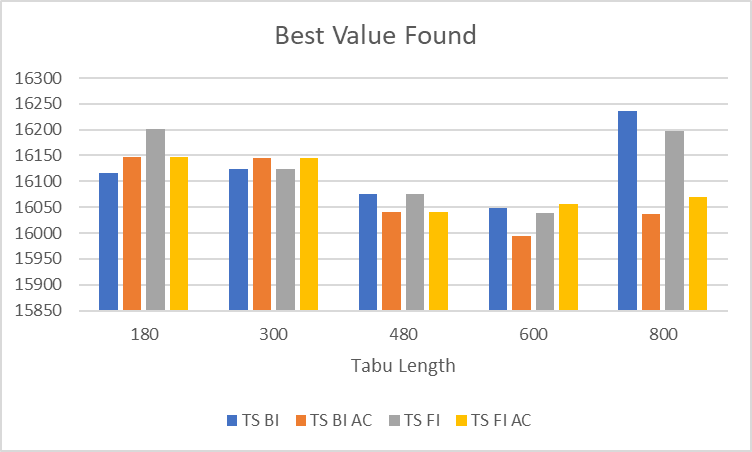
\includegraphics[width=\linewidth]{img/RI-calibration-SC-2}
			
			\vspace{1cm}
			
			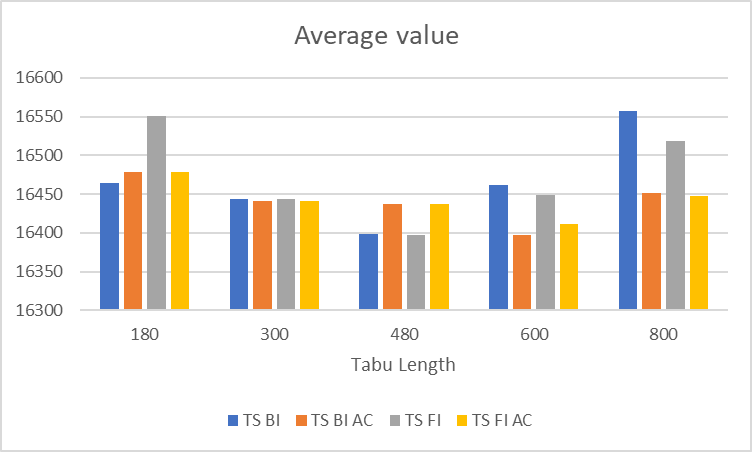
\includegraphics[width=\linewidth]{img/RI-calibration-SC-avg-2}
			
			\caption{Calibration Real Instances (code optimize).}
			\label{fig:ri-calibration-sc-opt}
		\end{figure}
	
	
		
			
		
		
			
			
		
			
		
			
			
			
	
	
	
		
		
	